\documentclass{beamer}

%----------------------------------------------------------------------------------------
%	PACKAGES
%----------------------------------------------------------------------------------------
\usepackage{caption}
\usepackage{amsmath}
\usepackage{amssymb}
\usepackage{tikz}
\usetikzlibrary{matrix,backgrounds,arrows,decorations.markings}
\tikzset{
  big arrow/.style={
    decoration={markings,mark=at position 1 with {\arrow[scale=2,#1]{>}}},
    postaction={decorate},
    shorten >=0.4pt,
    dashed=true},
  big arrow/.default=red,
  }
%----------------------------------------------------------------------------------------

\mode<presentation> {
\usetheme{Montpellier}

\setbeamertemplate{footline}{
  \leavevmode%
  \hbox{%
  \begin{beamercolorbox}[wd=.4\paperwidth,ht=2.25ex,dp=1ex,center]{mb2244}%
    \usebeamerfont{mb2244}\insertshortauthor
  \end{beamercolorbox}%
  \begin{beamercolorbox}[wd=.8\paperwidth,ht=2.25ex,dp=1ex,center]{title in head/foot}%
    \insertframenumber{} / \inserttotalframenumber\hspace*{1ex}
  \end{beamercolorbox}}%
  \vskip0pt%
}

% Remove the navigation symbols from the bottom slides
\setbeamertemplate{navigation symbols}{}
}

%----------------------------------------------------------------------------------------
%	TITLE PAGE
%----------------------------------------------------------------------------------------

\title{Collapsing Heterogeneous Towers of Interpreters}

\author[mb2244]{Michael Buch -- mb2244}
\institute
{
University of Cambridge\\ % Your institution for the title page
\medskip
}
\date{\today} % Date, can be changed to a custom date

\begin{document}

\begin{frame}
\titlepage % Print the title page as the first slide
\end{frame}

\begin{frame}
\frametitle{Overview} % Table of contents slide, comment this block out to remove it
\tableofcontents % Throughout your presentation, if you choose to use \section{} and \subsection{} commands, these will automatically be printed on this slide as an overview of your presentation
\end{frame}

% Show table of contents on section change
\AtBeginSection[]
{
\begin{frame}{Table of Contents}
\tableofcontents[currentsection]
\end{frame}
}

\newcommand{\mslang}{$\lambda_{\uparrow\downarrow}$}

%----------------------------------------------------------------------------------------
%	PRESENTATION SLIDES
%----------------------------------------------------------------------------------------
\section{Towers of Interpreters}
\begin{frame}{What are they?}
  \begin{columns}
    \begin{column}{0.5\textwidth}
      \begin{itemize}
        \item Reflective Towers
        \item E.g.: 3-LISP, Brown, Blond
        \item n-fold interpretative overhead
      \end{itemize}
    \end{column}
    \begin{column}{0.5\textwidth}
      \begin{figure}
        \centering
        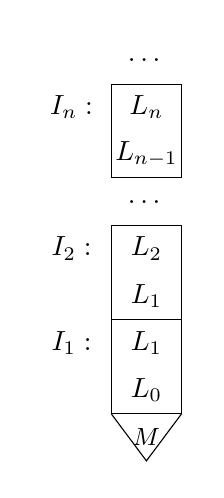
\begin{tikzpicture}
          \matrix (m) [matrix of nodes,nodes={minimum width=2.5em,minimum  height=1.7em},ampersand replacement=\&]
            {
                        \& \dots                   \\
                $I_n:$  \& $L_n$                   \\
                        \& $L_{n-1}$               \\
                        \& \dots                   \\
                $I_2:$  \& $L_2$                   \\
                        \& $L_1$                   \\
                $I_1:$  \& $L_1$                   \\
                        \& $L_0$                   \\
                        \& |[font=\small]|$M$      \\
              };
              \draw (m-1-2.south west) |- (m-4-2.north east) |- (m-1-2.south west);
              \draw (m-4-2.south west) |- (m-6-2.south east) |- (m-4-2.south west);
              \draw (m-4-2.south west) |- (m-8-2.south east) |- (m-6-2.north east);
              \draw (m-8-2.south west) -- (m-9-2.south) -- (m-8-2.south east);
        \end{tikzpicture}
      \end{figure}
    \end{column}
  \end{columns}
\end{frame}

\begin{frame}{Black/Pink}
Collapsing towers
\end{frame}

\begin{frame}{Motivating Example}
  \begin{columns}
    \begin{column}{0.5\textwidth}
      \begin{itemize}
        \item Python on x86 JavaScript emulator
        \item Different internal structure to reflective towers e.g. bytecode
        \item Need some way of expressing this \textit{generalization}
      \end{itemize}
    \end{column}
    \begin{column}{0.5\textwidth}
      \begin{figure}
        \centering
        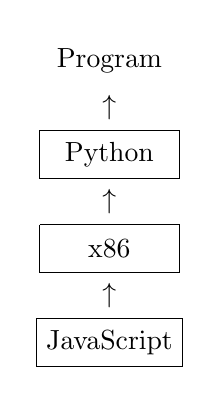
\begin{tikzpicture}
          \matrix (m) [matrix of nodes,nodes={minimum width=5em,minimum  height=1.7em},ampersand replacement=\&]
            {
              Program                   \\
              $\uparrow$                \\
              Python                    \\
              $\uparrow$                \\
              x86                       \\
              $\uparrow$                \\
              JavaScript                \\
              };
              \draw (m-3-1.north west) |- (m-3-1.south east) |- (m-3-1.north west);
              \draw (m-5-1.north west) |- (m-5-1.south east) |- (m-5-1.north west);
              \draw (m-7-1.north west) |- (m-7-1.south east) |- (m-7-1.north west);
        \end{tikzpicture}
      \end{figure}
    \end{column}
  \end{columns}
\end{frame}

\section{Heterogeneity}
\begin{frame}{Heterogeneous Towers}
    \begin{itemize}
        \item Can be non-meta-circular
        \item Can have semantic gap
    \end{itemize}
\end{frame}

\section{Project Aims}
\begin{frame}{Aims}
    \begin{itemize}
        \item Construct and collapse heterogeneous towers of interpreters
        \item Explore effects of heterogeneity on collapse procedure
    \end{itemize}
\end{frame}

\begin{frame}{Methodology}
      \begin{columns}
    \begin{column}{0.5\textwidth}
    \begin{itemize}
        \item Construct a tower resembling PYTHON-X86-JS DIAGRAM
        \item Similar to motivating example, internal structure is different to those of reflective towers
    \end{itemize}
    \end{column}
    \begin{column}{0.5\textwidth}
      \begin{figure}
        \centering
        \begin{tikzpicture}
          \matrix (m) [matrix of nodes,nodes={minimum width=5em,minimum  height=1.7em},ampersand replacement=\&]
            {
              Program                   \\
              $\uparrow$                \\
              META                      \\
              $\uparrow$                \\
              SECD                      \\
              $\uparrow$                \\
              \mslang                   \\
              };
              \draw (m-3-1.north west) |- (m-3-1.south east) |- (m-3-1.north west);
              \draw (m-5-1.north west) |- (m-5-1.south east) |- (m-5-1.north west);
              \draw (m-7-1.north west) |- (m-7-1.south east) |- (m-7-1.north west);
        \end{tikzpicture}
      \end{figure}
    \end{column}
  \end{columns}
\end{frame}

\section{Background}
\begin{frame}{Type-Directed Partial Evaluation}
\end{frame}
\begin{frame}{\texorpdfstring{\mslang}{}}
\end{frame}
\section{Collapsing a Tower}
\begin{frame}{Ingredients}
    \begin{itemize}
        \item Multi-level Language
        \item Stage Polymorphism
        \item TDPE-style Lift
    \end{itemize}
\end{frame}
\section{Experimental Tower}
% lift: Problems in its construction and staging at different levels
%   Non-termination of TDPE
% Show example collapse

\section{Summary}
\begin{frame}{Conclusions}
\end{frame}
\begin{frame}{Future Work}
\end{frame}

\begin{frame}
\Huge{\centerline{mb2244}}
\end{frame}

\end{document}
